% !TeX program = xelatex

\documentclass{beamer}
\usepackage{fontspec}
\usepackage{outlines}
\usepackage{transparent}

\usetheme{metropolis}
\usecolortheme[snowy]{owl}
\definecolor{constructiveTitle}{HTML}{fbb4da}
\setbeamercolor{frametitle}{parent=normal, bg=constructiveTitle}
\graphicspath{{../}}

\renewcommand{\r}{\rightarrow}
\newcommand{\N}{\mathbb{N}}


\title{Konstruktiivinen logiikka ja formaali todistaminen}
\subtitle{0 – Johdanto}
\author{Niklas Halonen \& Alma Nevalainen}

\begin{document}
\addtocounter{framenumber}{-1}

\frame{\titlepage}

\begin{frame}
  \frametitle{Esittely}
  Tällä tunnilla selviää:
  \begin{itemize}
    \item Kurssin käytänteet, aiheet ja tavoitteet
    \item Mitä on (konstruktiivinen) logiikka
    \item Mitä on matematiikka
    \item Miten todistaa, että $\sqrt 2$ on irrationaalinen
    \item Mitä \emph{todistaminen} edes tarkoittaa
  \end{itemize}
\end{frame}

\begin{frame}
  \frametitle{Kurssin käytänteet}
  \begin{itemize}
    \item MA ja KE 8-palkki (15.00 – 16.15)
    \item Ei arvosanaa, S-merkintä
    \item Läpipääsy vaatii, että tekee joka \emph{maailmasta} vähintään puolet tehtävistä
    \item Kotitehtäviä tulee jonkin verran :)
  \end{itemize}
\end{frame}

\begin{frame}
  \frametitle{Kurssin aiheet}
  \begin{enumerate}
    \item[0.] Matemaatiikan määritelmät
    \item Lauselogiikka
    \item Todistaminen
    \item Formaali logiikka $\bot \vdash 4 = 5$
    \item Aritmetiikka, $\N$
    \item Funktiot, $\N \r \N$
    \item Joukot, $\{2n \mid n \in \N\}$
  \end{enumerate}
\end{frame}

\begin{frame}
  \frametitle{Kurssin tavoitteet}
  \begin{outline}
    \1 Ymmärtää lause- ja predikaattilogiikan perusteet
      \2 Mitä on totuusarvot
      \2 Totuus ja epätotuus
      \2 Implikaatio
      \2 Konjunktio, disjunktio
      \2 Negaatio
    \1 Tietää 1900-luvun vaihteessa joukko-oppia piinaavia paradokseja
    \1 Tietää tyyppiteorian perusteet
      \2 Tyypit
      \2 Todistustermit
    \1 Ymmärtää luonnollisten lukujen konstruktion ja induktioperiaatteen
    \1 Osaa induktiivista päättelyä
    \1 Tietää miten matematiikkaa formalisoidaan tietokoneavusteisesti Leanillä
  \end{outline}
\end{frame}

\begin{frame}
  \frametitle{Mitä on logiikka}
  \begin{outline}
    \1 Filosofian haara
    \1 Kieli, jossa lauseet vastaavat "korrektia" päättelyä
      \2 "Mars on punainen" \emph{ja} "Mars on planeetta" \\ \emph{seuraa} "Mars on punainen planeetta"
      \2 "Mars on sininen" \emph{ja} "Mars on planeetta" \\ \emph{seuraa} "Mars on sininen planeetta"
    \1 Perusta matematiikalle (Logisismi)
    \1 $A \land (\neg A \lor B) \Rightarrow B = 1$
    \1 $\forall x, \text{lentävä\_lintu}(x) \to \text{lentää}(x)$
  \end{outline}
\end{frame}

{
\setbeamertemplate{background canvas}
    {%
        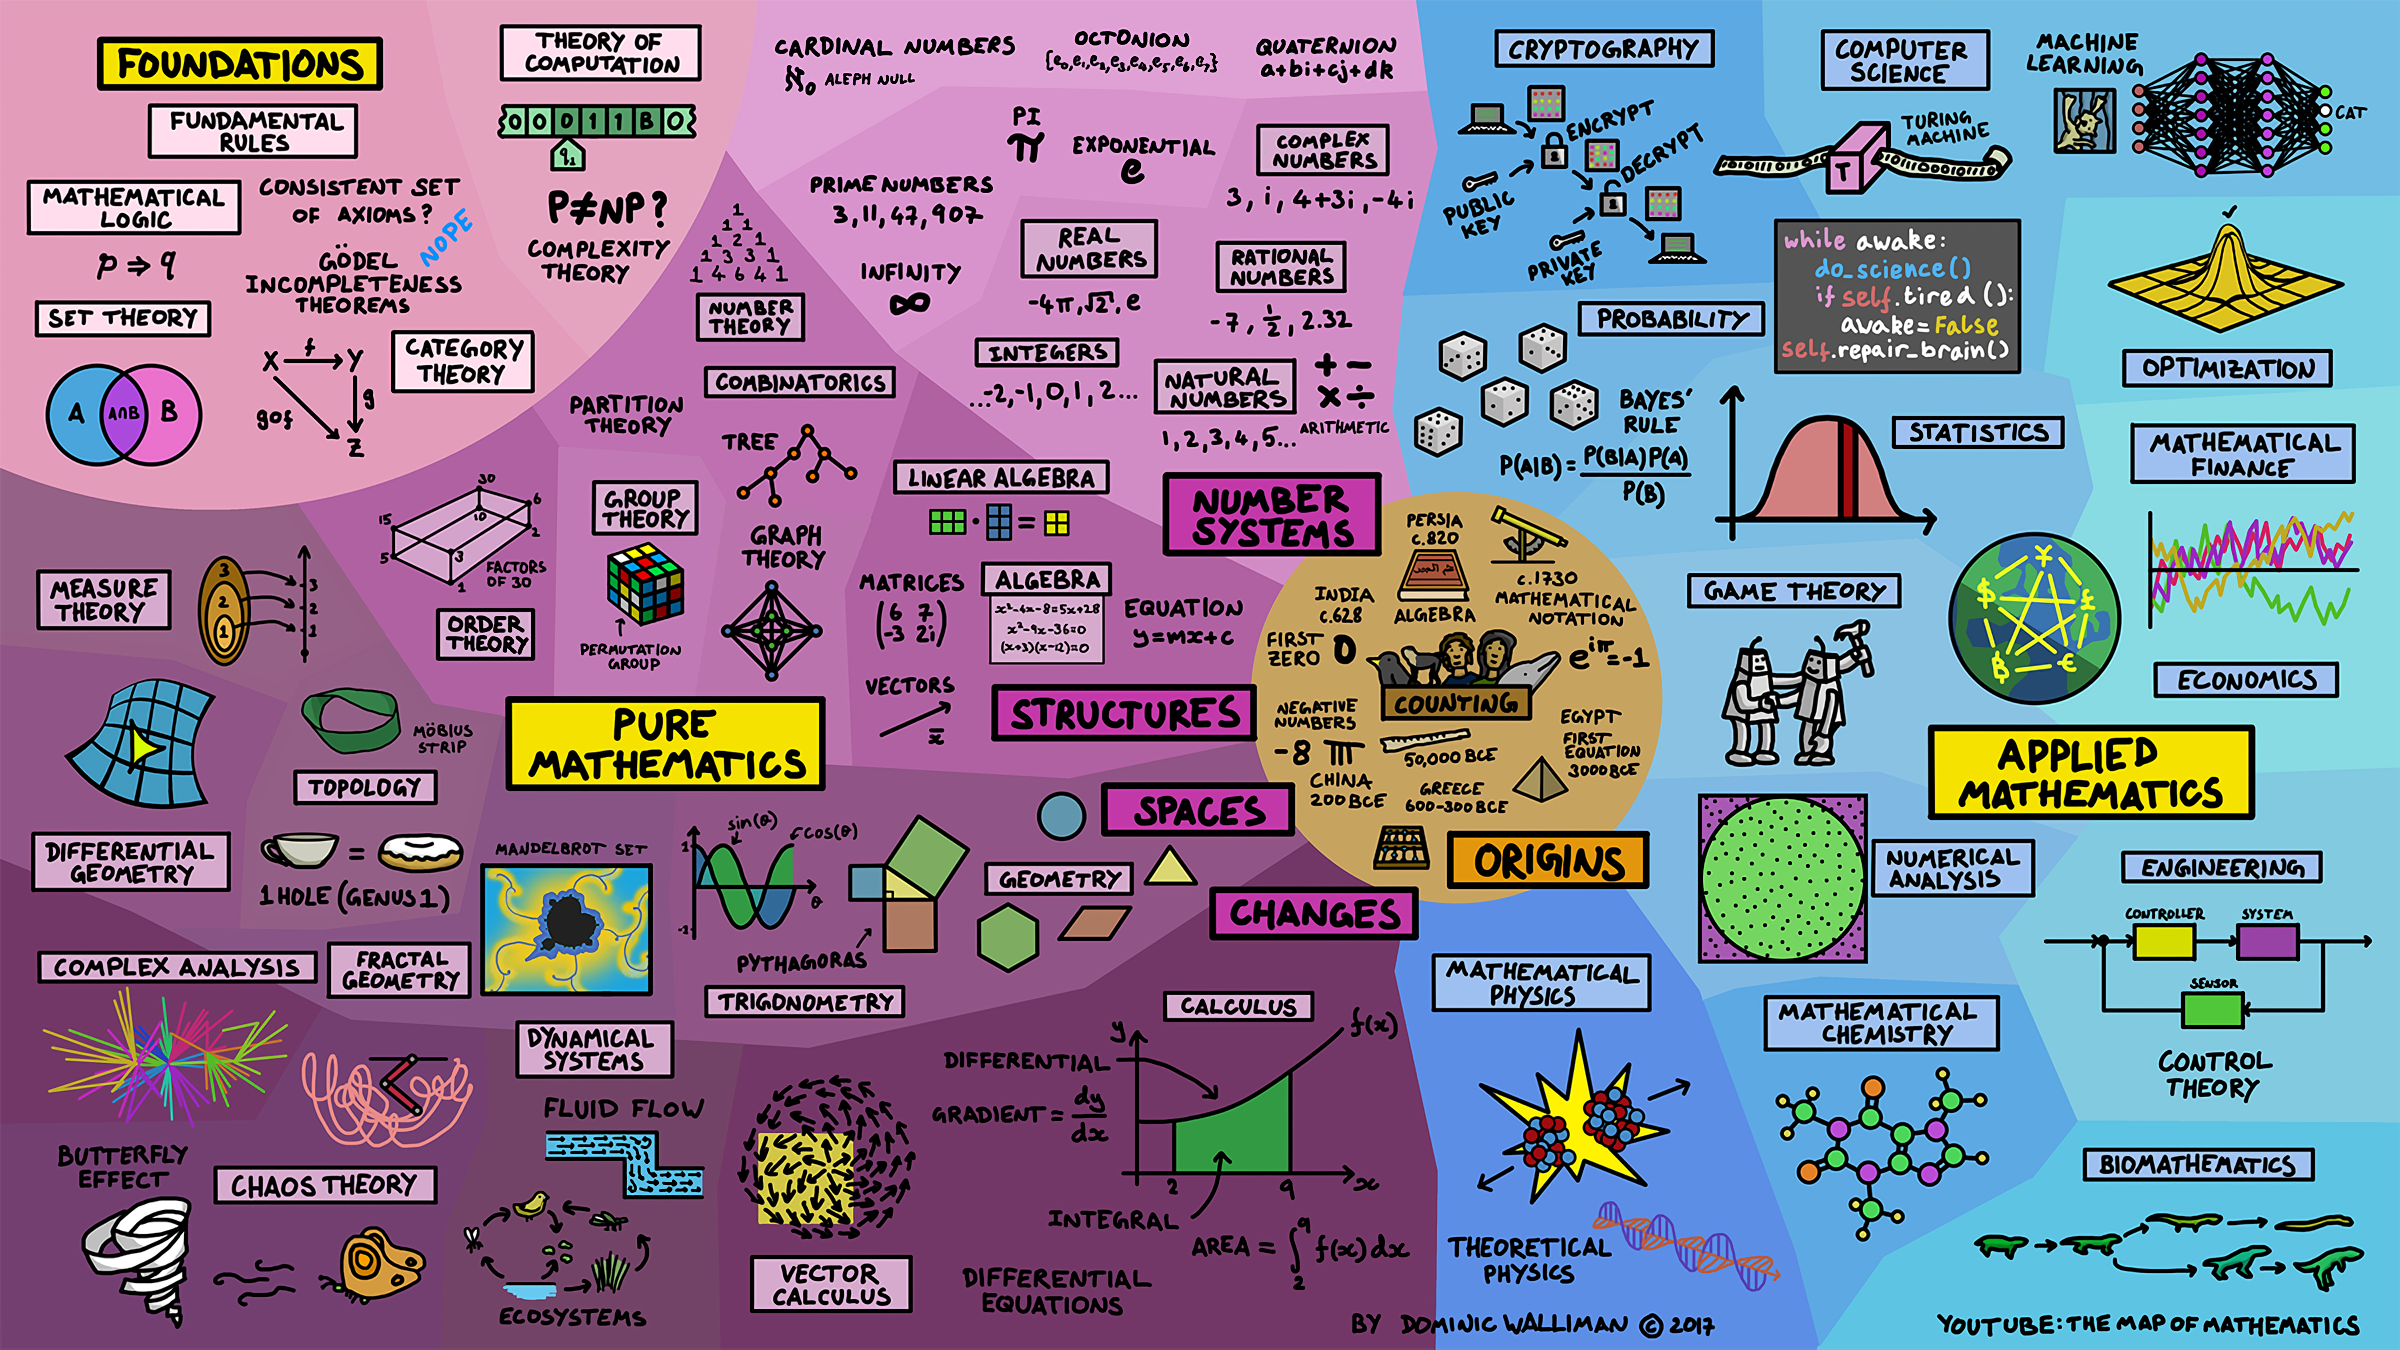
\includegraphics[width=\paperwidth,height=\paperheight]{./docs/static/map.png}
    }
\begin{frame}
\end{frame}
}

\begin{frame}
  \frametitle{Mitä on matematiikka}

\end{frame}

\begin{frame}
  \frametitle{Mitä on todistaminen}

\end{frame}

\end{document}
